%----------------------------------------------------------------------------------------
%    PACKAGES AND THEMES
%----------------------------------------------------------------------------------------

\documentclass[aspectratio=169,xcolor=dvipsnames]{beamer}
\usetheme{SimpleDarkBlue}

\usepackage{hyperref}
\usepackage{graphicx} % Allows including images
\usepackage{booktabs} % Allows the use of \toprule, \midrule and \bottomrule in tables

%----------------------------------------------------------------------------------------
%    TITLE PAGE
%----------------------------------------------------------------------------------------

\title{Generating Parkinson’s Disease gait patterns using Generative Adversarial Network}
\subtitle{Neurodegenerative Diseases}

\author{Fleșar Radu}

\institute
{
    West University of Timișoara
}
\date{\today} % Date, can be changed to a custom date

%----------------------------------------------------------------------------------------
%    PRESENTATION SLIDES
%----------------------------------------------------------------------------------------

\begin{document}

\begin{frame}
    % Print the title page as the first slide
    \titlepage
\end{frame}

%------------------------------------------------
\section{First Section}
%------------------------------------------------

\begin{frame}{Data Collection}
\begin{itemize}
    \item \textbf{Wearable physiograph}
    \begin{itemize}
        \item Three plantar pressure sensors for each leg:
        \begin{itemize}
            \item Below the toe
            \item Metatarsal arch
            \item Heel area
        \end{itemize}
        \item Two EMG channels for each leg that acquire:
        \begin{itemize}
            \item Tibialis anterior muscle activity
            \item Gastrocnemius medialis muscle activity
        \end{itemize}
        \item Accelerometer mounted on subject’s wrist
    \end{itemize}
    \item \textbf{16 subjects in the study group}
    \begin{itemize}
        \item 12 patients
        \item 3 healthy controls
        \item 1 suspect
    \end{itemize}
\end{itemize}

\end{frame}

%------------------------------------------------

\begin{frame}{Image Generation}
\begin{figure}
    \centering
    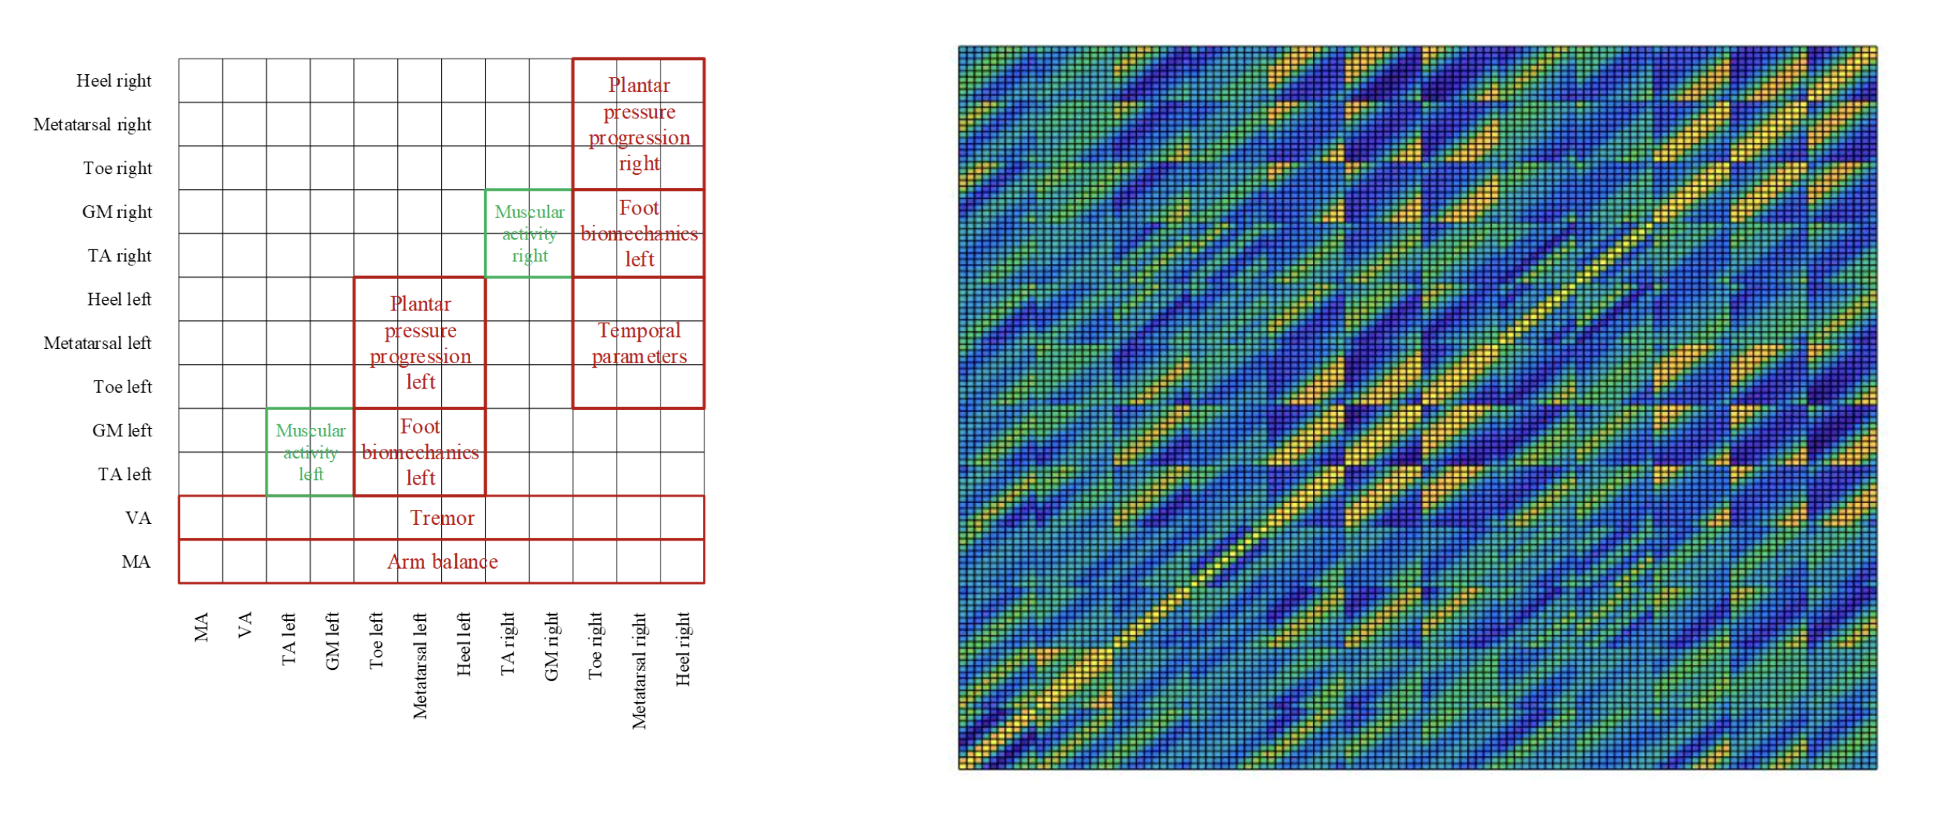
\includegraphics[width=0.95\linewidth]{image.png}
    \caption{Image Generation Scheme and Example}
    \label{fig:enter-label}
\end{figure}
\end{frame}

%------------------------------------------------

\begin{frame}{Old Dataset}
    \begin{figure}
        \centering
        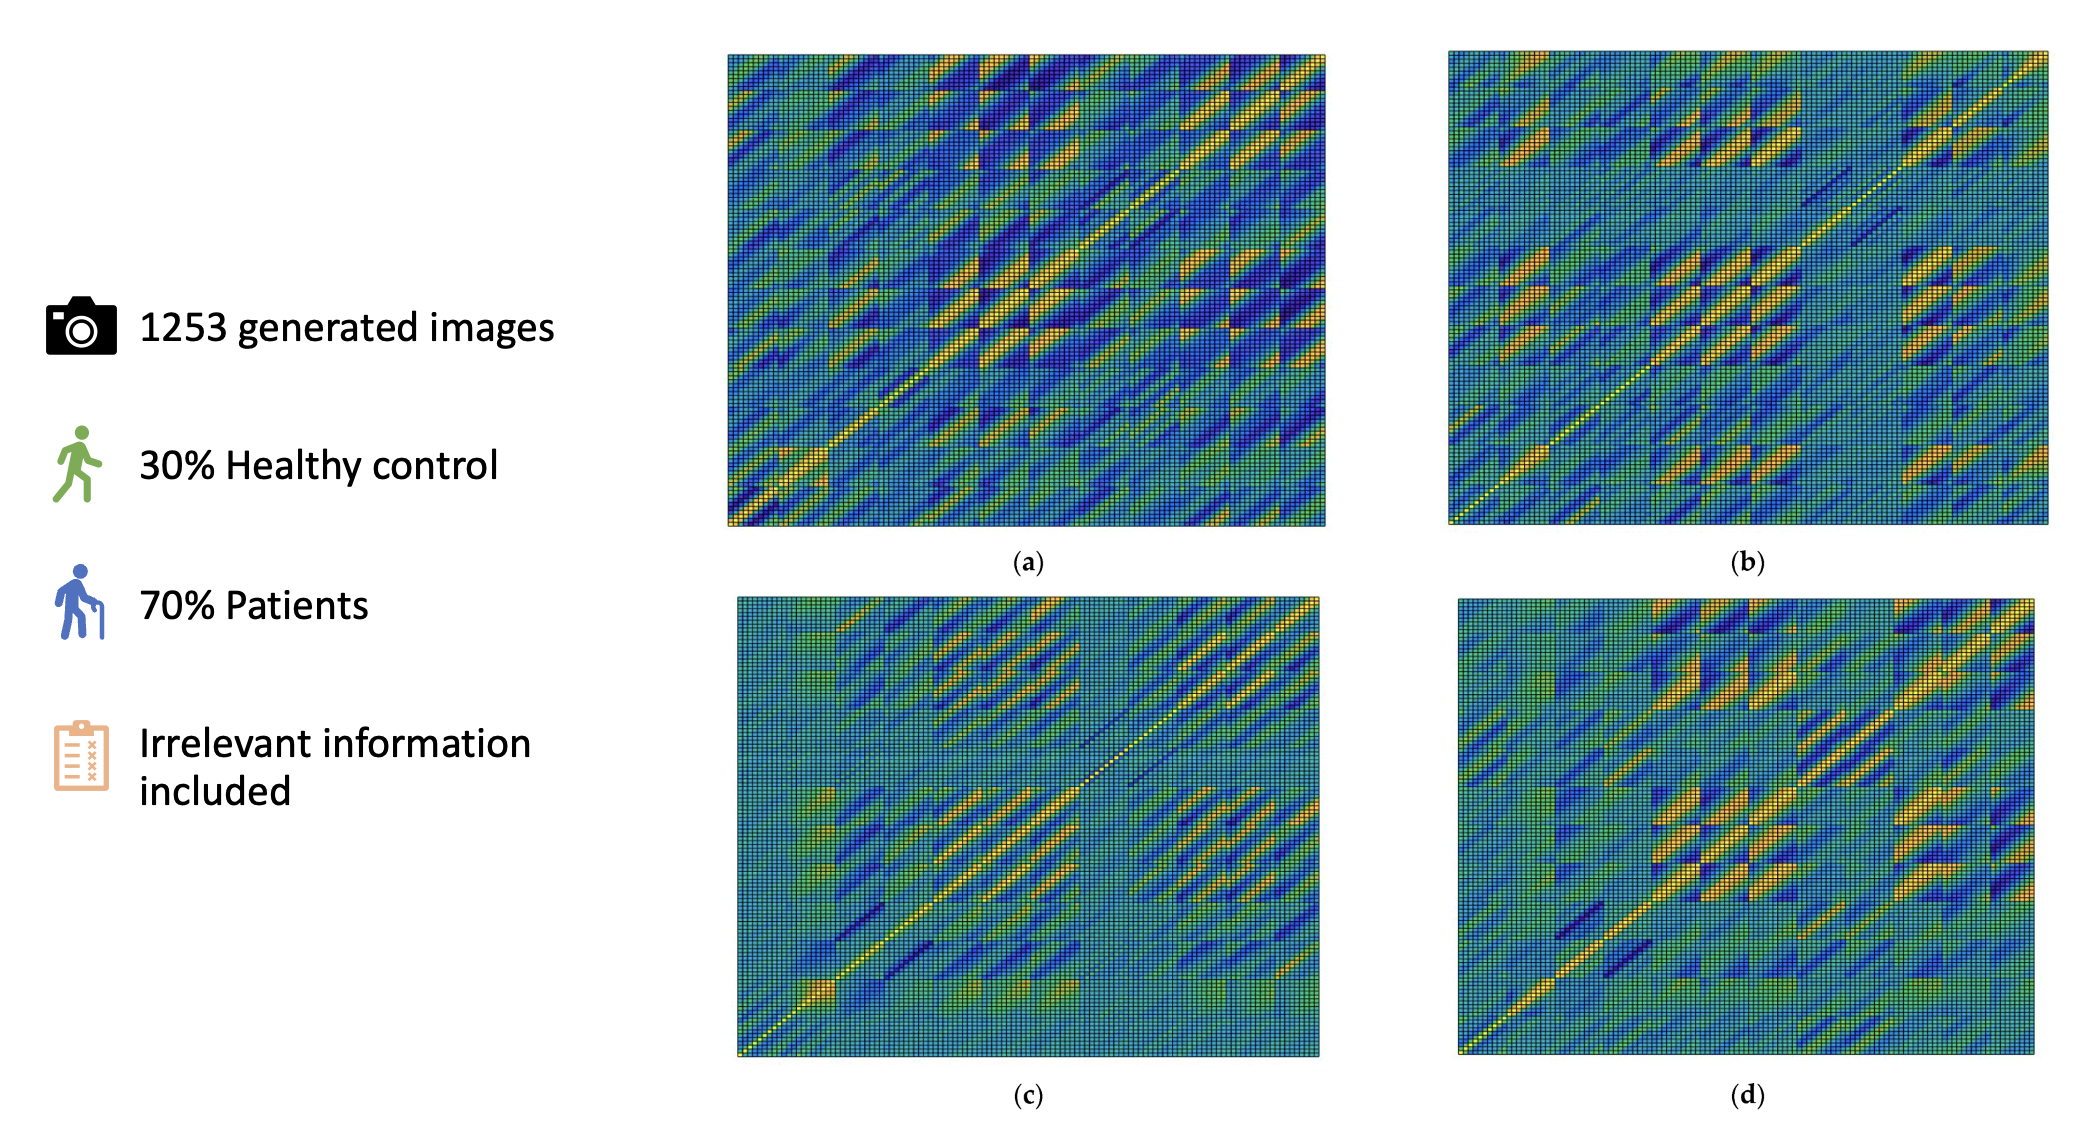
\includegraphics[width=0.99\linewidth]{Screenshot 2025-02-25 at 18.20.25.png}
        \caption{Enter Caption}
        \label{fig:enter-label}
    \end{figure}
\end{frame}


\begin{frame}{AI Decisional Support}
    \begin{figure}
        \centering
        
\includegraphics[width=0.99\linewidth]{models.png}
    \end{figure}
\end{frame}

\begin{frame}{Training metrics}

    \begin{figure}
        \centering
        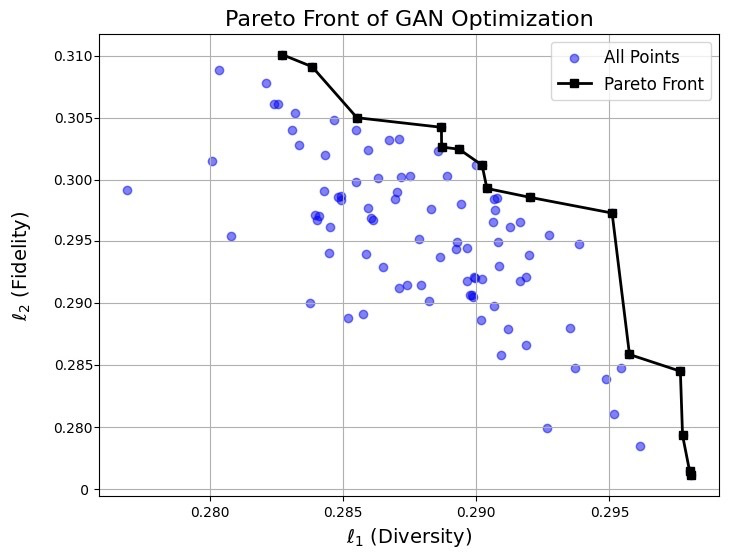
\includegraphics[width=0.7\linewidth]{pareto.png}
    \end{figure}
\end{frame}

\begin{frame}{Evolution}
    \begin{figure}
        \centering
        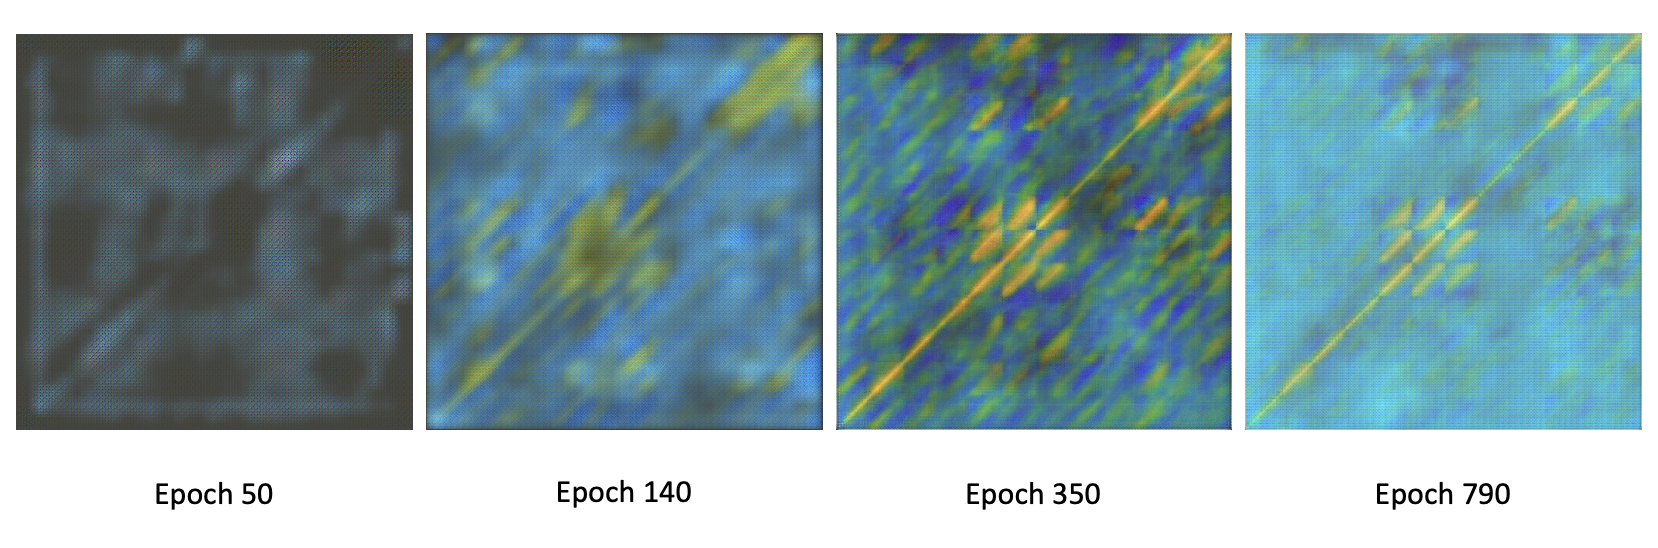
\includegraphics[width=0.95\linewidth]{ganEvol.png}
    \end{figure}
\end{frame}


\begin{frame}{Results}
    \begin{figure}
        \centering
        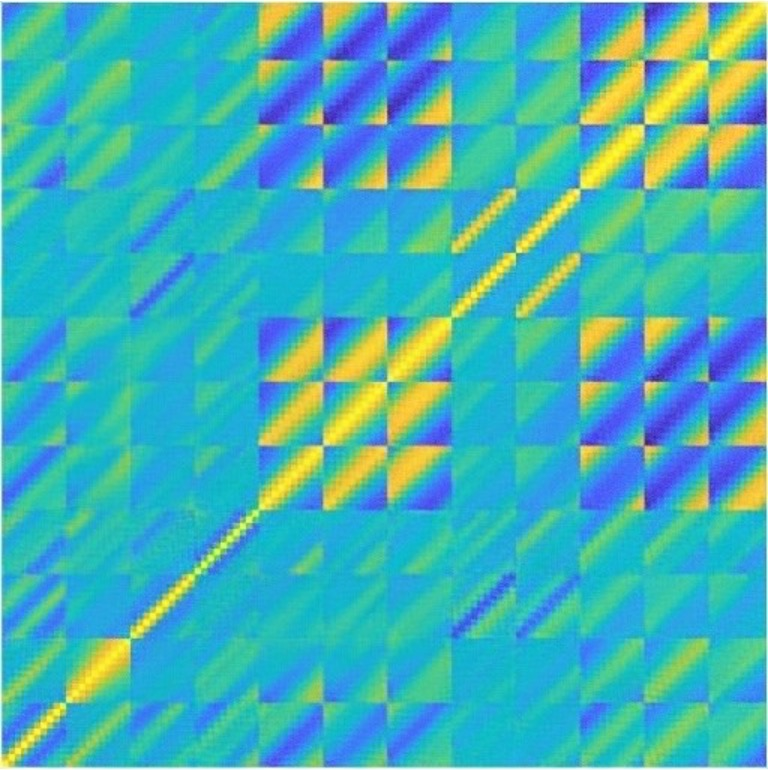
\includegraphics[width=0.35\linewidth]{result.jpeg}
        \caption{Results after 40000 epochs}
        \label{fig:enter-label}
    \end{figure}
\end{frame}
%------------------------------------------------


\end{document}